\documentclass[12pt]{report} % Type du document
\usepackage[french]{babel} % Langue du document
\usepackage[T1]{fontenc}
\usepackage[utf8]{inputenc}
\usepackage[left=15mm, right=15mm]{geometry} % Définition de la largeur des marges gauches et droites

\usepackage{a4wide} % Format de la feuille
\usepackage{amsmath} % Pour inclure des équations
\usepackage{graphicx} % Pour inclure des images / graphiques
\usepackage{float} % Pour gérer le placement des images
\usepackage{fancyhdr} % Pour les headers, paramètres ci-dessous
\usepackage{listings} %Pour afficher du code formaté
\usepackage{subcaption}

\graphicspath{ {images/} }

% Paramètres fancyhdr
\pagestyle{fancy}
\rhead{Basile Botebol, Baptiste Hardrick}
\lhead{
\includegraphics[width=1.5cm]{HEIG.png}}
\cfoot{\thepage} % thepage affiche le numéro de page courant
\setlength{\parindent}{0cm}

\title{\textbf{SOS 2019\\Securité Des OS\\Laboratoire 1 - Windows}} % '\\' force un retour à la ligne (Bonne pratique: Réserver ça aux titres)
\author{Basile Botebol, Baptiste Hardrick\\Groupe 6}
\date{Mai 2019} % Laisser vide pour ne pas afficher la date 


\begin{document}

\maketitle

\section*{Reconnaissance}

\subsection*{Réponses aux questions}
\paragraph{P1 :} -Pn traite tous les hôtes comme étant en ligne -> cela permet de passer outre la découverte des hôtes

\paragraph{P2 :} WAD-DC-SRV2\\
On peut le déterminer en faisant les manipulations présentées dans le laboratoire (en scannant le port 445 (smb)) 
et en regardant leur nom (celui dont le nom comporte DC)\\
La deuxième méthode se fait en scannant grâce à un nmap sur port 88 car c'est sur ce port que tourne kerberos qui est 
propre au domain controler.


\subsection*{Résultat des Manipulations}

\begin{figure}[!h]
	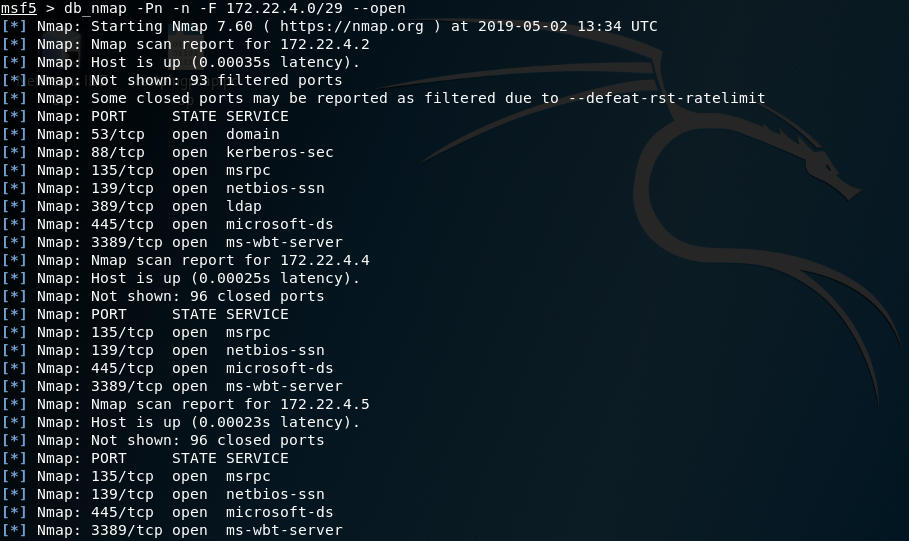
\includegraphics[width=17cm]{db_nmap_3_1_a.PNG}
	\caption*{Résultat du db nmap - partie 1}
\end{figure}

\begin{figure}
	\newpage
	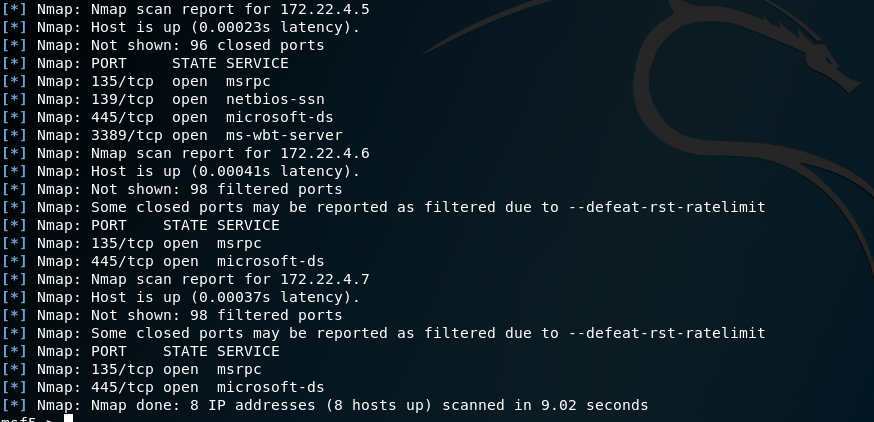
\includegraphics[width=17cm]{db_nmap_3_1_b.PNG}
	\caption*{Résultat du db nmap - partie 2}
\end{figure}

\newpage
~
\newpage

\section*{Exploitation de vulnérabilités logicielles}

\subsection*{Réponses aux questions}
\paragraph{P3 :} ip vulnérable: 172.22.4.6\\
On obtient les droits d'exécution SYSTEM
\paragraph{P4 :}  La faille MS17-010 permet à l'attaquant d'exécuter n'importe quelle commande et donc, d'avoir les privilèges system.
\paragraph{P5 :} 188 powershell.exe (grâce aux commandes getpid et ps dans le meterpreter)
\paragraph{P6 :} Un reverse shell fait en sorte que la victime vienne se connecter à un port définit par l'attaquant (sur sa machine) alors qu'un bind shell consiste à ouvrir un port sur la machine de la victime et à s'y connecter.
\paragraph{P7 :} Il est recommandé d'utiliser un reverse shell lorsqu'il y a un firewall protégeant la victime (ce qui risquerait d'empêcher un bind)
\paragraph{P8 :} Il s'agit de composants payload (comme Meterpreter dans notre cas) qui sont téléchargés depuis un Stager.
Les Stagers permettant eux de créer une connection entre l'attaquant et la victime.

\newpage
\subsection*{Résultat des Manipulations}

\begin{figure}[!h]
	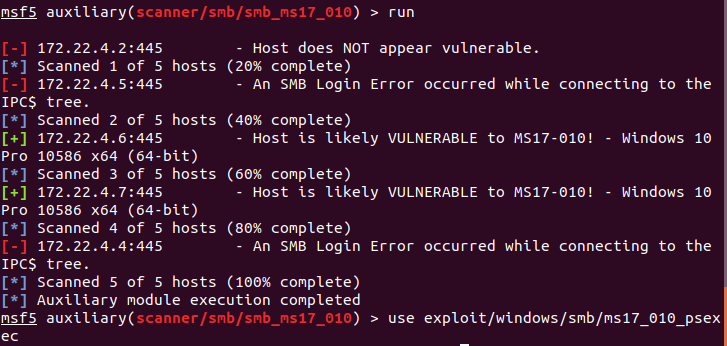
\includegraphics[width=17cm]{3_2-Scann.PNG}
	\caption*{Résultat du scan}
\end{figure}

\begin{figure}[!h]
	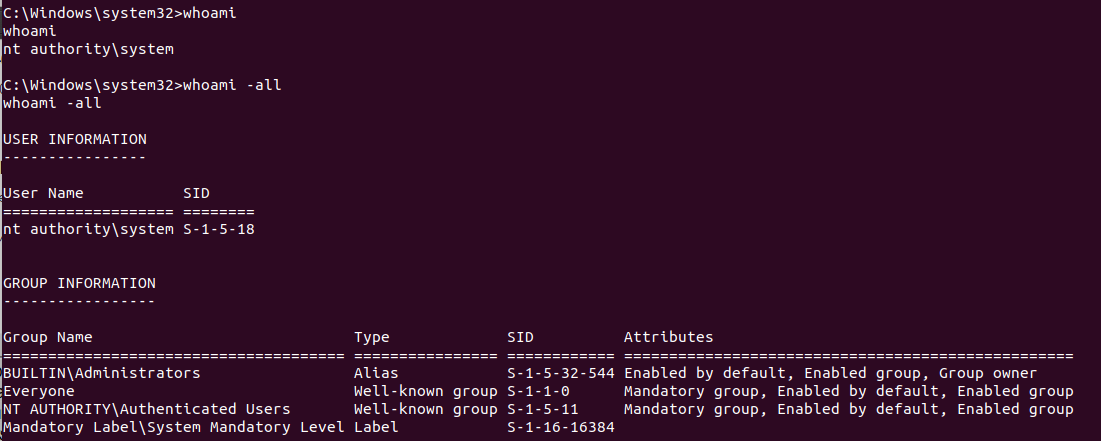
\includegraphics[width=17cm]{who_am_i_3_2.PNG}
	\caption*{Savoir quel compte on a obtenu avec whoami}
\end{figure}


\begin{figure}[!h]
	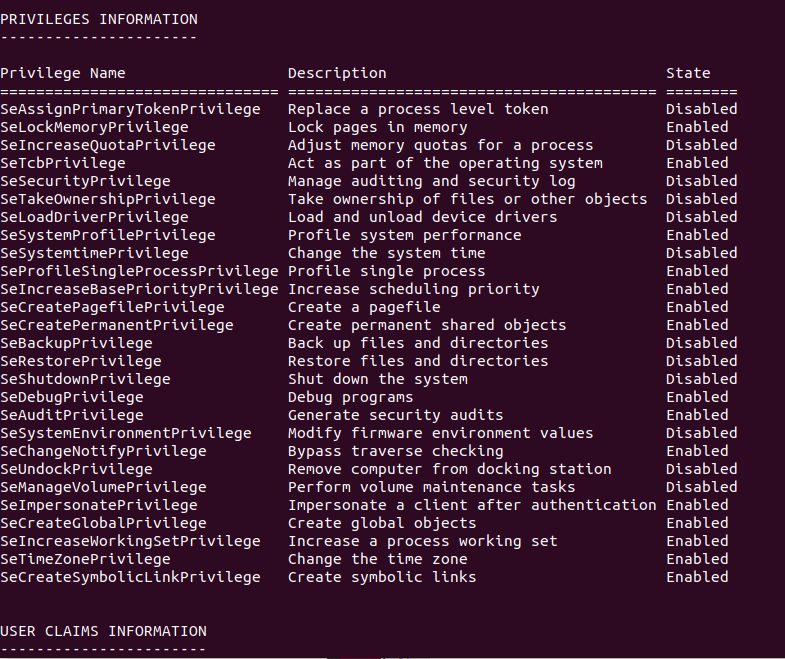
\includegraphics[width=17cm]{Privileges_3_2.PNG}
	\caption*{Liste des privilèges obtenus}
\end{figure}


\newpage
~
\newpage

\section*{Vol de credentials}

\subsection*{Réponses aux questions}

\paragraph{P9 :}	Il est composé ainsi: username : userid : lm hash : ntlm hash
\paragraph{P10 :} Le LM hash étant désactivé, il est toujours à la même valeur, soit la valeur trouvée : aad3b435b51404eeaad3b435b51404ee
Les comptes guest et default account ont également le même ntlm hash (soit : 31d6cfe0d16ae931b73c59d7e0c089c0), ce qui semble indiquer que ces deux comptes n'ont pas de mot de passe (les noms des compte guest et default account semblent aller dans ce sens)

\paragraph{P11 :} Oui, les deux desktop utilisent le même compte administrator, et toutes les machines partagent les deux autres comptes (sans pouvoir se connecter cependant)

\paragraph{P12 :} Le format du hash est comme suit:  MD4( MD4(password) + username))\\
Les différentes parties sont: la version du ms-cache (ici DCC2), l'id du groupeauquel appartient l'utilisateur,  le username et enfin le hash
\paragraph{P13 :} C'est pour signifier qu'il s'agit d'une compte machine
\paragraph{P14 :} Il faut avoir les droits system pour accèder au GPO sur sysvol (c'est-à-dire ouvrir un meterpreter via ms17\_010\_psexec et non via smb/psexec comme on a pu l'essayer)
\paragraph{P15 :} Oui, le 'utilisateur svc\_sched et le mot de passe K33pAlive4ever sont utilisables sur les machines suivantes
(voir la figure ci-dessous)
\paragraph{P16 :} 
\paragraph{P17 :} Oui, voir capture

\newpage
\subsection*{Résultat des Manipulations}

\begin{figure}[!h]
	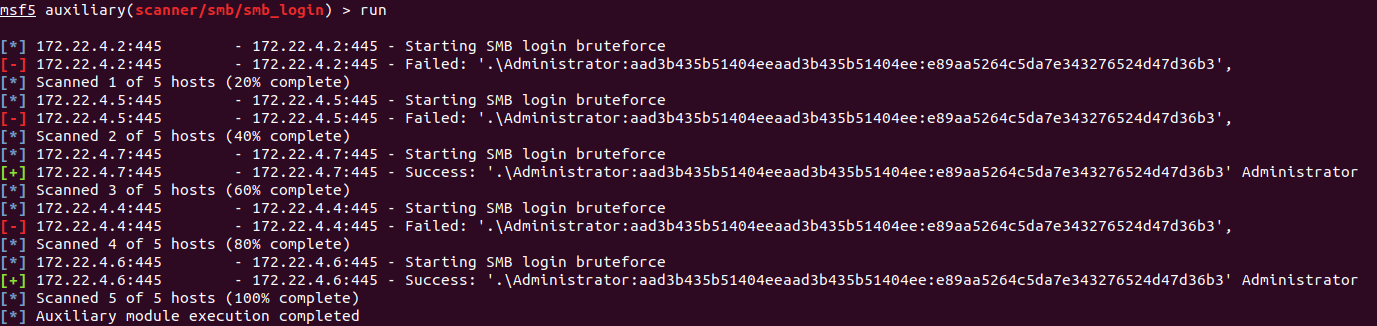
\includegraphics[width=17cm]{P11-a.PNG}
	\caption*{Résultat du scan (P11) - partie 1}
\end{figure}

\begin{figure}[!h]
	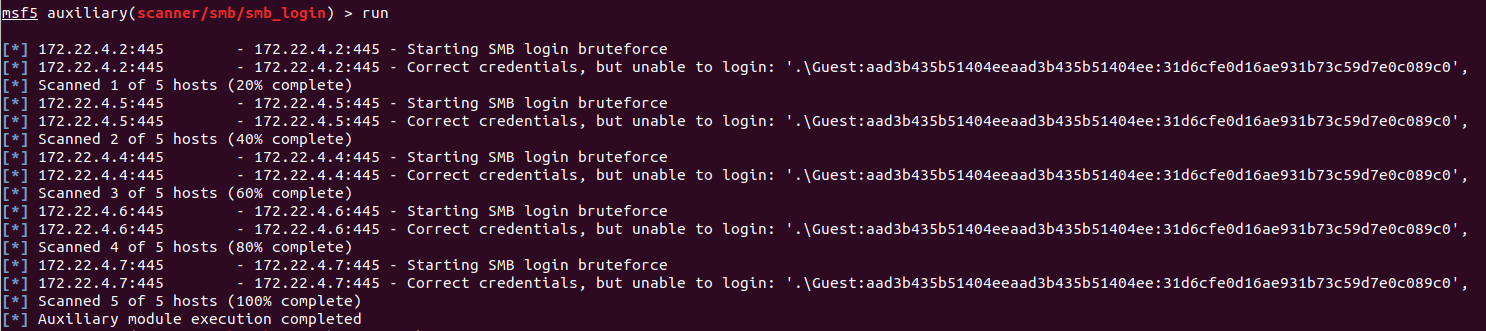
\includegraphics[width=17cm]{P11-b.PNG}
	\caption*{Résultat du scan (P11) - partie 2}
\end{figure}

\begin{figure}[!h]
	\includegraphics[width=17cm]{P11-c.PNG}
	\caption*{Résultat du scan (P11) - partie 3}
\end{figure}

\begin{figure}[!h]
	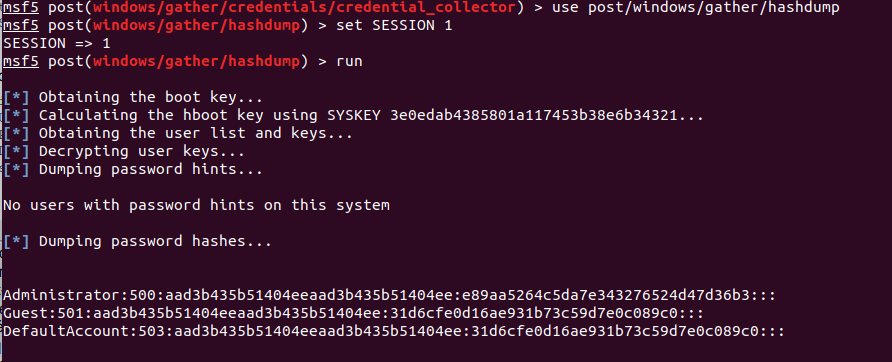
\includegraphics[width=17cm]{hashdump_SAM_3_3.PNG}
	\caption*{Résultat du hashdump montrant le contenu de la SAM}
\end{figure}

\begin{figure}[!h]
	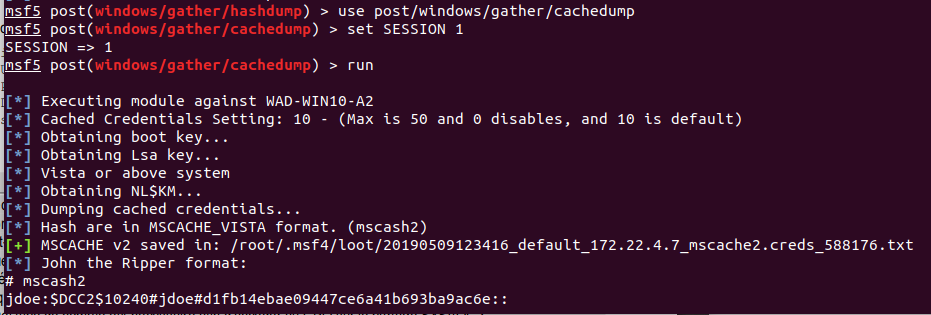
\includegraphics[width=17cm]{mscash_3_3.PNG}
	\caption*{Contenu du MS-CACHE}
\end{figure}

\begin{figure}[!h]
	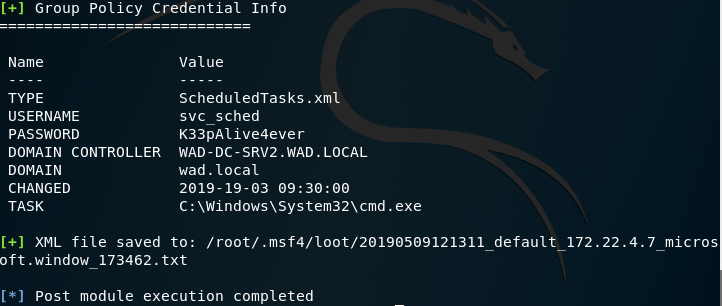
\includegraphics[width=17cm]{3_3_gather_credentials.PNG}
	\caption*{Résultat du GPP contenant les credentials}
\end{figure}

\begin{figure}[!h]
	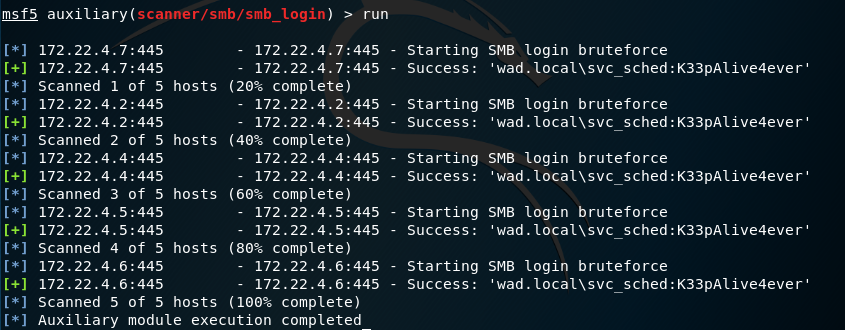
\includegraphics[width=17cm]{3_3_reused_passwords.PNG}
	\caption*{Résultat du test de réutilisation de mot de passe sur d'autres machines (P15-P17)}
\end{figure}


\newpage
~
\newpage
~
\newpage

\section*{Kerberoast}

\subsection*{Réponses aux questions}
\paragraph{P18 :} get\_user\_spns renvoie une seule entrée, car un seul arbitrary spn (MSSQL) a été trouvé. Les arbitrary spn ont en général un mot de passe plus court (car défini par l'utilisateur) et quasiment jamais changé (car devant être changé par l'utilisateur).
\paragraph{P19 :} MSSQLSvc/WAD-SQLSRV01.WAD.local:1433
\paragraph{P20 :} adm-sql avec le mot de passe Andromeda1
\paragraph{P21 :} Oui, voir capture d'écran


\subsection*{Résultat des Manipulations}

\begin{figure}[!h]
	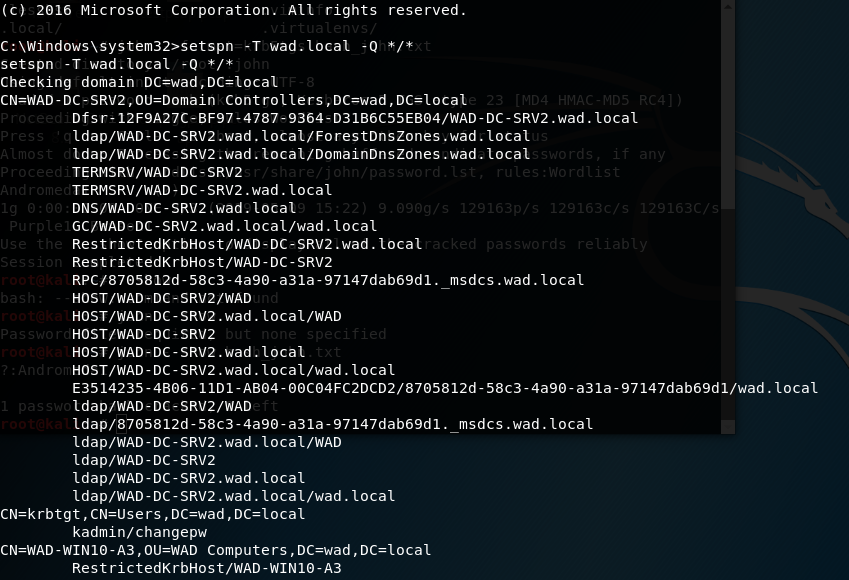
\includegraphics[width=17cm]{SPN_command_a.PNG}
	\caption*{Résultat de ls recherche des SPN - partie 1}
\end{figure}

\begin{figure}[!h]
	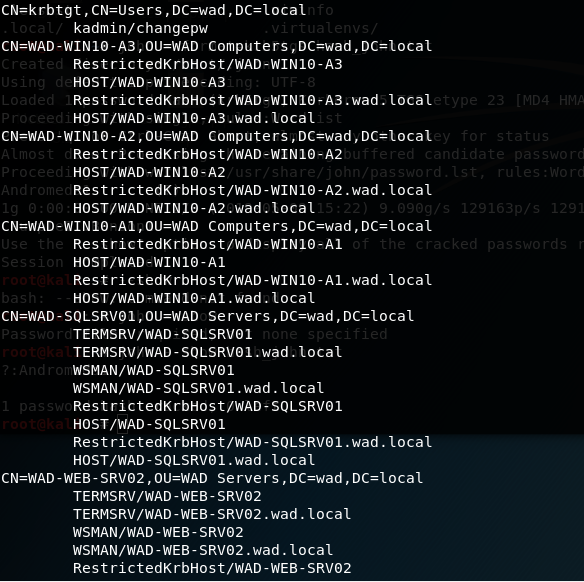
\includegraphics[width=17cm]{SPN_command_b.PNG}
	\caption*{Résultat de ls recherche des SPN - partie 2}
\end{figure}

\begin{figure}[!h]
	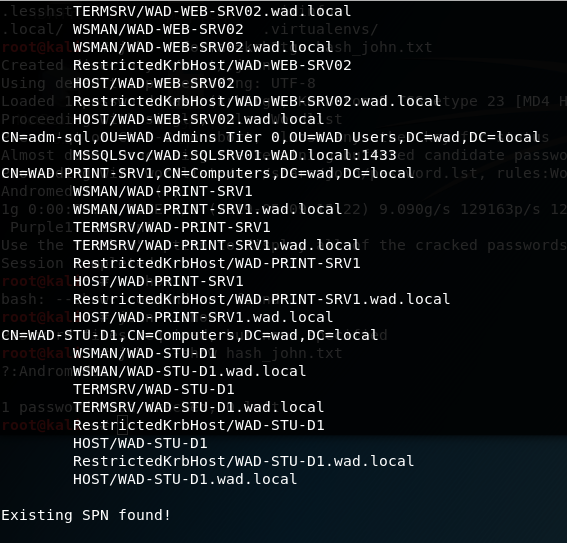
\includegraphics[width=17cm]{SPN_command_c.PNG}
	\caption*{Résultat de ls recherche des SPN - partie 3}
\end{figure}

\begin{figure}[!h]
	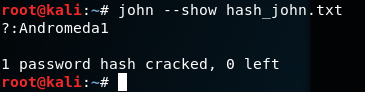
\includegraphics[]{password_john_cracked.PNG}
	\caption*{Résultat du crack john the ripper}
\end{figure}

\begin{figure}[!h]
	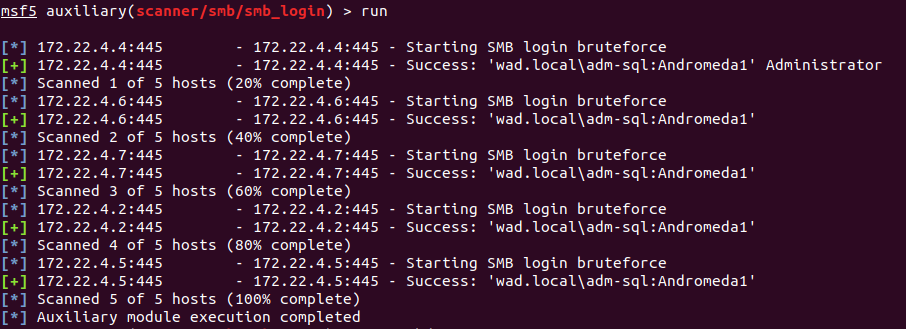
\includegraphics[width=17cm]{P21.PNG}
	\caption*{Résultat du smb\_login (P21)}
\end{figure}


\newpage
~
\newpage
~
\newpage
\section*{Mouvements latéraux}

\subsection*{Réponses aux questions}
\paragraph{P22 :}
\paragraph{P23 :} Il  faut des privilèges administrateurs car psexec lance des services Windows et il faut être admin pour le faire
\paragraph{P24 :} On utilise pass the hash (la vulnérabilité est que pour l'authentification ne nécessite pas le mot de passe, mais le hash du mot de passe)
\paragraph{P25 :} Après avoir exécuté load kiwi puis creds\_all 
\paragraph{P26 :} Pour des configurations larges sur tous les domaines, pour promouvoir des utilisateurs en admin, etc
\paragraph{P27 :} En empêchant l'accès à l'ordinateur qui contient le Domain Admin depuis le réseau par exemple

\newpage
\subsection*{Résultat des Manipulations}


\begin{figure}[!h]
	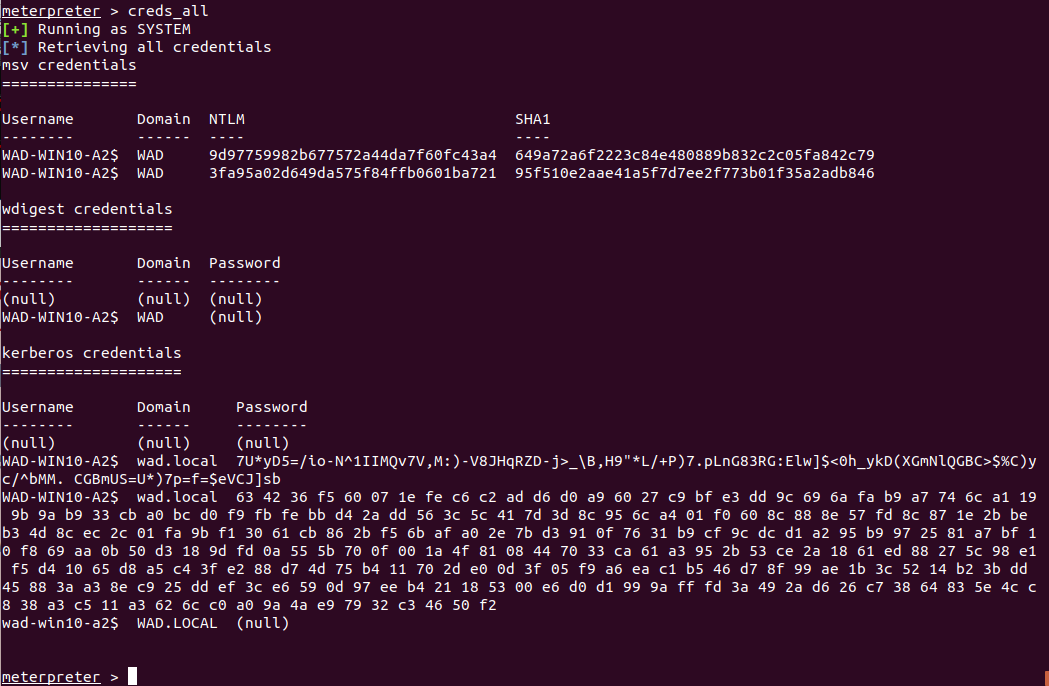
\includegraphics[width=17cm]{mimikatz_creds_all.PNG}
	\caption*{Résultat Mimikatz sur adm-sql}
\end{figure}

\begin{figure}[!h]
	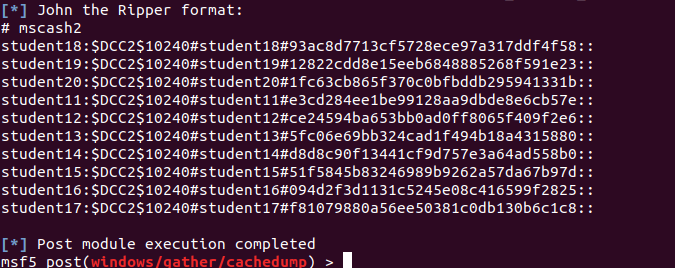
\includegraphics[width=17cm]{cachedump_server_5_3-5.PNG}
	\caption*{Résultat cachedump sur adm-sql}
\end{figure}

\begin{figure}[!h]
	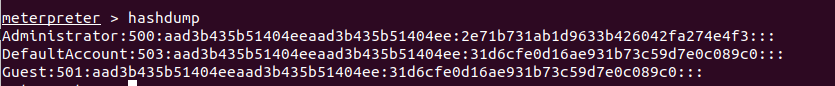
\includegraphics[width=17cm]{hashdump_sql_server3-5.PNG}
	\caption*{Résultat hashdump sur adm-sql}
\end{figure}

\begin{figure}[!h]
	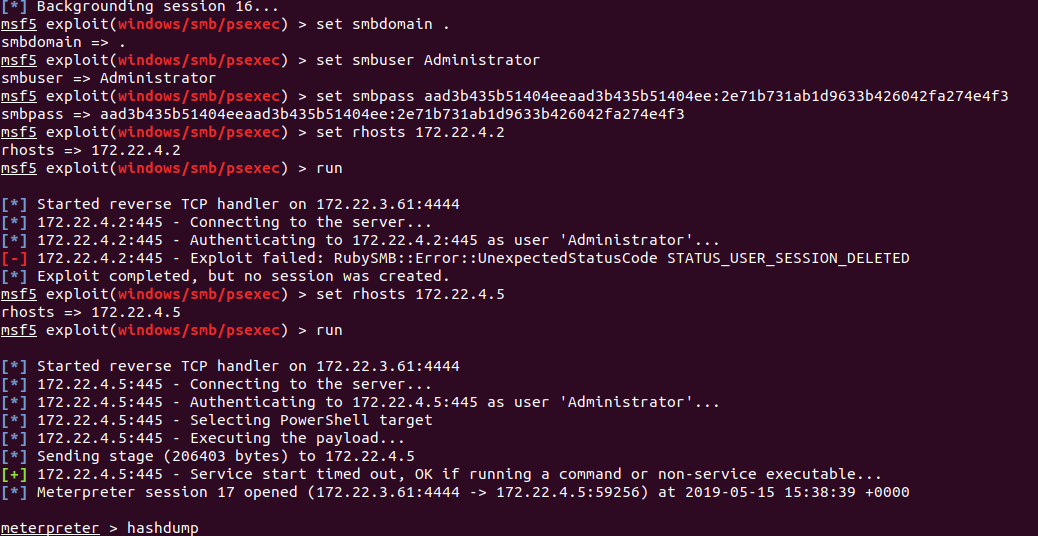
\includegraphics[width=17cm]{pass_the_hash_first_3-5.PNG}
	\caption*{Premier pass the hash}
\end{figure}

\begin{figure}[!h]
	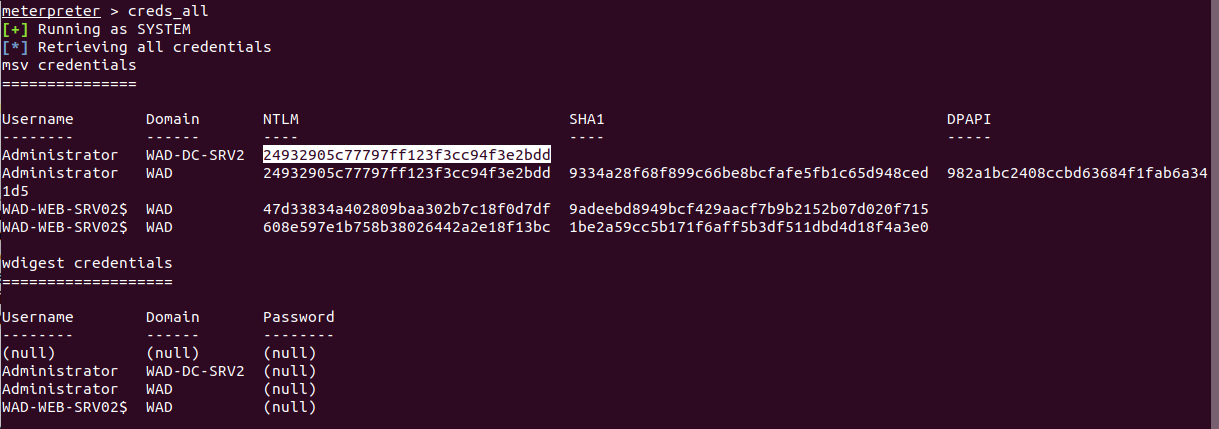
\includegraphics[width=17cm]{creds_all_server5_3-5.PNG}
	\caption*{Résultat Mimikatz sur cet Administrator}
\end{figure}

\begin{figure}[!h]
	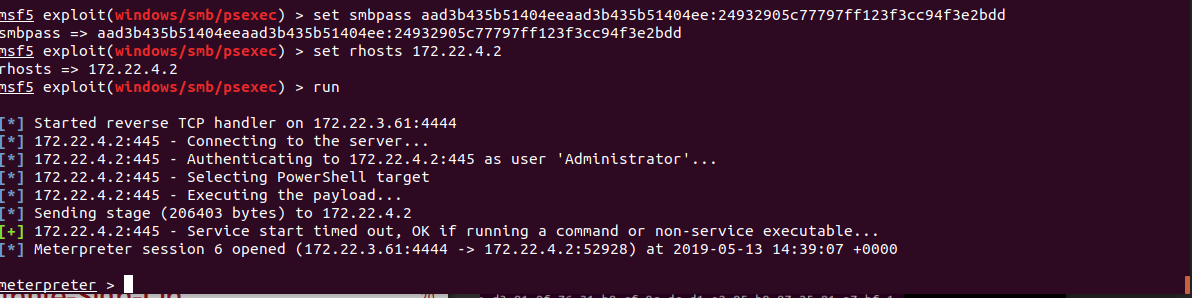
\includegraphics[width=17cm]{3_5_loginSMB_172_22_4_2.PNG}
	\caption*{Accès au domain admin}
\end{figure}

\begin{figure}[!h]
	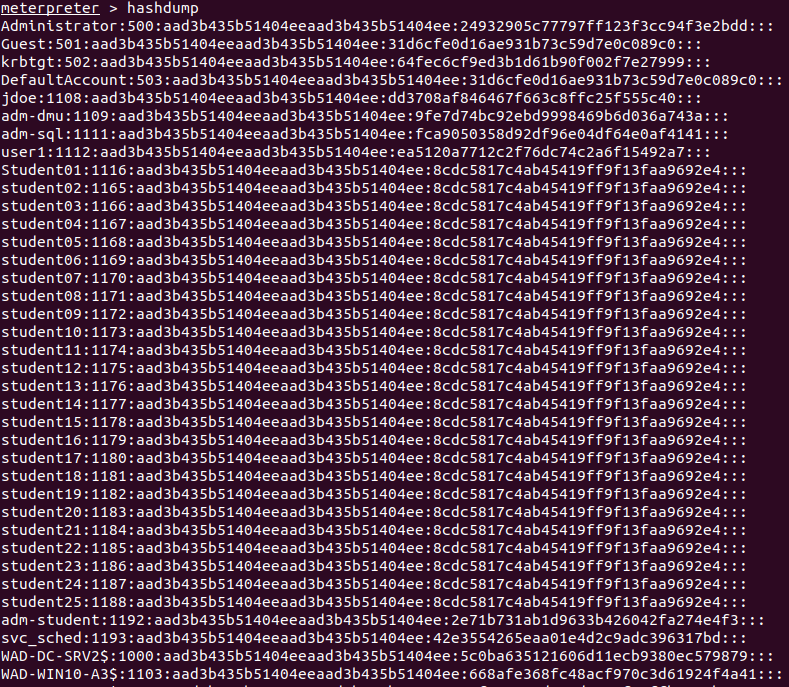
\includegraphics[width=17cm]{hashdump_3_5_1_sur_2.PNG}
	\caption*{Hashdump du domain admin - partie 1}
\end{figure}

\begin{figure}[!h]
	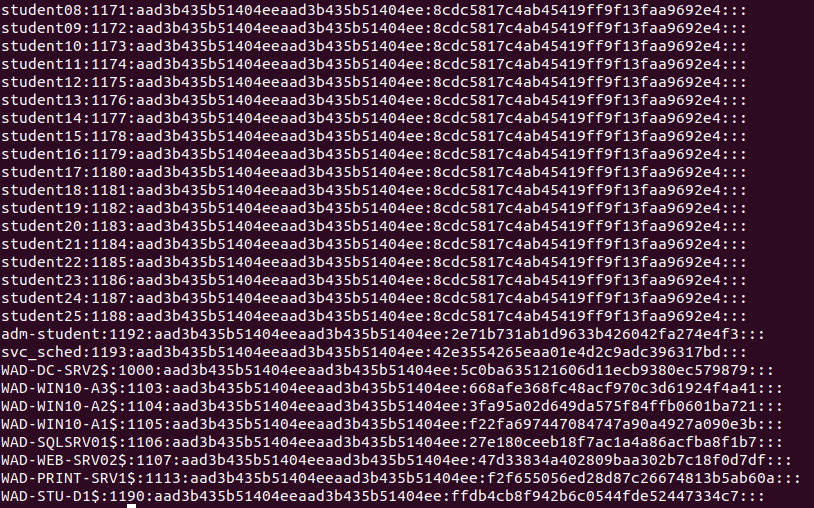
\includegraphics[width=17cm]{hashdump_3_5_2_sur_2.PNG}
	\caption*{Hashdump du domain admin - partie 2}
\end{figure}

\newpage
~
\newpage
~
\newpage
~
\newpage
\section*{Persistance}

\subsection*{Réponses aux questions}
\paragraph{P28 :} On reçoit un system error comme quoi on n'est pas log avec un utilisateur ayant les bons privilèges
\paragraph{P29 :} La seconde fois le système nous le permet. En forgeant le golden ticket, on a accès aux droits de tous les utilisateurs,
y compris celui du Domain Admin, ce qui nous donne le droit de faire ce qu'on veut sur cette machine, y compris monter un partage.
\paragraph{P30 :} On voit plusieurs événements avec l'ID 4624, ce qui signifie qu'on s'est bien connecté (avec notre compte)
\paragraph{P31 :} Le golden ticket a la même durée de vie que le DC
\paragraph{P32 :}  Surveiller l'activité lié au golden ticket (c'est-à-dire son utlisateur). Ou refaire tout le domaine.

\subsection*{Résultat des Manipulations}

\begin{figure}[!h]
	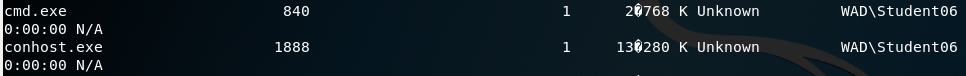
\includegraphics[width=17cm]{3_6_process_used_by_us.PNG}
	\caption*{process utilisé par notre utilisateur (no 6) - se trouve dans la seconde colonne}
\end{figure}

\begin{figure}[!h]
	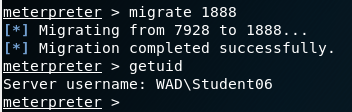
\includegraphics[]{3_6_migrate.PNG}
	\caption*{migration effective}
\end{figure}

\begin{figure}[!h]
	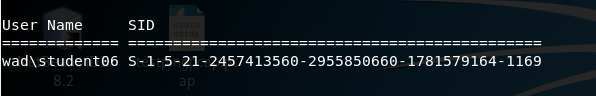
\includegraphics[]{3_6_domain_SID.PNG}
	\caption*{connaitre le domain SID}
\end{figure}

\begin{figure}[!h]
	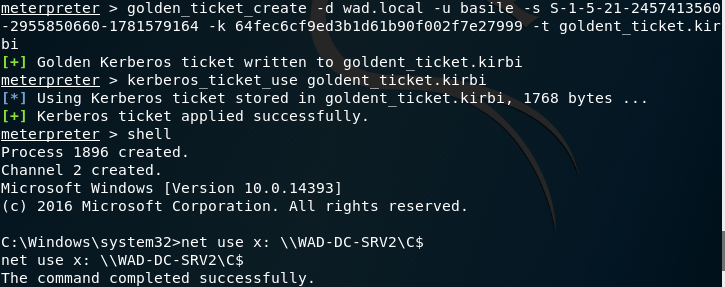
\includegraphics[width=17cm]{3_6_golden_ticket_works.PNG}
	\caption*{création d'un golden ticket valide et mount validé}
\end{figure}

\begin{figure}[!h]
	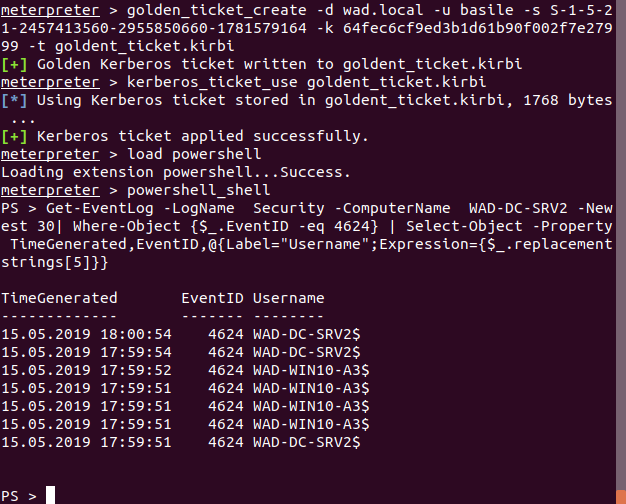
\includegraphics[width=17cm]{p30_logs_powershell.PNG}
	\caption*{Logs powershell (réponse à P30)}
\end{figure}

\end{document}



